\documentclass[conference]{IEEEtran}
\IEEEoverridecommandlockouts
% The preceding line is only needed to identify funding in the first footnote. If that is unneeded, please comment it out.
\usepackage{cite}
\usepackage{amsmath,amssymb,amsfonts}
\usepackage{graphicx}
\usepackage{textcomp}

\usepackage{algorithm}
\usepackage[noend]{algpseudocode}
\usepackage{subfigure}
\usepackage{multirow}
\usepackage[hidelinks]{hyperref}


\usepackage{bbold}

\renewcommand{\algorithmicrequire}{\textbf{Input:}}
\renewcommand{\algorithmicensure}{\textbf{Output:}}

\def\BibTeX{{\rm B\kern-.05em{\sc i\kern-.025em b}\kern-.08em
    T\kern-.1667em\lower.7ex\hbox{E}\kern-.125emX}}
    
\bibliographystyle{IEEEtran}
\usepackage[show]{chato-notes}

\newcommand{\E}[1]{\cdot10^{#1}}

\let\oldReturn\Return
\renewcommand{\Return}{\State\oldReturn}

\renewcommand{\citedash}{--} 
    
\begin{document}

\title{SNM: Stochastic Newton Method for Optimization of Discrete Choice Models}

\author{

\IEEEauthorblockN{Gael Lederrey}
\IEEEauthorblockA{\small \textit{Transport and Mobility Laboratory} \\
\textit{\'Ecole Polytechnique F\'ed\'erale de Lausanne}\\
Station 18, CH-1015 Lausanne \\
\texttt{gael.lederrey@epfl.ch}}
\and
\IEEEauthorblockN{Virginie Lurkin}
\IEEEauthorblockA{\small \textit{Transport and Mobility Laboratory} \\
\textit{\'Ecole Polytechnique F\'ed\'erale de Lausanne}\\
Station 18, CH-1015 Lausanne \\
\texttt{virginie.lurkin@epfl.ch}}
\and
\IEEEauthorblockN{Michel Bierlaire}
\IEEEauthorblockA{\small \textit{Transport and Mobility Laboratory} \\
\textit{\'Ecole Polytechnique F\'ed\'erale de Lausanne}\\
Station 18, CH-1015 Lausanne \\
\texttt{michel.bierlaire@epfl.ch}}
}

\maketitle

\begin{abstract}
Optimization algorithms are rarely mentioned in the discrete choice literature. One reason may be that classic Newton-Raphson methods have been rather successful in estimating discrete choice parameters on available data sets of limited size. However, thanks to recent advances in data collection, abundant data about choice situations become more and more available, and state-of-the-art algorithms can be computationally burdensome on these massive datasets.  In this paper, inspired by the good practices from the machine learning field, we introduce a Stochastic Newton Method (SNM) for the estimation of discrete choice models parameters. Our preliminary results indicate that our method outperforms (stochastic) first-order and quasi-newton methods. 
\end{abstract}

\begin{IEEEkeywords}
Discrete Choice Models, Optimization
\end{IEEEkeywords}

\section{Introduction}
\label{sec:intro}

Discrete choice models (DCM) have become an essential operational tool in modeling individual behavior. Many success stories have been reported in the scientific studies in transportation, marketing, health, or economics, among others. Estimating the parameters of those models requires to solve an optimization problem and yet, optimization algorithms are rarely mentioned in the discrete choice literature. One reason may be that classic nonlinear optimization algorithms (i.e., Newton-Raphson method) have been rather successful in estimating discrete choice parameters on available data sets of limited size. Thanks to recent advances in data collection, abundant data about choice situations become more and more available. While offering a rich potential for a better understanding of human choices, these new data sources also bring new challenges for the community. Indeed algorithms classically embedded in state-of-the-art discrete choice software's (such as Biogeme~\cite{bierlaire_biogeme:_2003} or Larch~\cite{newman_computational_2018}) can be computationally burdensome on these massive datasets. 

In contrast, extracting useful information from big data sets is at the core of Machine Learning (ML). Primarily interested in achieving high prediction accuracy, ML algorithms (and especially Neural Networks)  have proved to be successful on models involving a huge number of parameters. Thus, large-scale machine learning models often involve both large volumes of parameters and large datasets. As such, first-order stochastic methods are a natural choice for large-scale machine learning optimization.  Due to the high cost of computing the full-Hessian, the second-order methods have been much less explored. And yet, algorithms exploiting second-order information can provide faster convergence. 

For the sake of interpretability, discrete choice models usually have a more restricted set of parameters than models typically investigated in the ML community. We, therefore, argue that it is possible to use second-order information to estimate these models. In this paper, inspired by the good practices and the intensive use of stochastic gradient methods in the ML field, we introduce a Stochastic Newton Method (SNM) for the estimation of discrete choice models parameters. The objective of this paper is to investigate the convergence of our algorithm by benchmarking it against standard first-order methods and quasi-newton methods using a simple logit model on a small dataset. We present preliminary results that indicate that our method outperforms (stochastic) first-order and quasi-newton methods. It constitutes a first step toward our final goal that is the development of an optimization method specifically designed to estimate discrete choice model parameters on big data sets.

The remainder of this paper is structured as follows. In section~\ref{sec:rel_work}, we present some related works about first and second-order optimization methods. In Section~\ref{sec:snm}, we describe the Stochastic Newton Method (SNM) algorithm that we propose. In Section~\ref{sec:case_study} we describe the discrete choice model we use, as well as the first-order methods and quasi-newton methods that we use as a benchmark to evaluate our algorithm. Section~\ref{sec:res} shows the results and we present our concluding remarks and future works in section~\ref{sec:conclusion}. 

\section{Related Work}
\label{sec:rel_work}

Optimization plays a crucial role in Machine Learning, especially for developing efficient and scalable algorithms suited for large datasets and complex models. In this respect, first-order methods have been extensively explored, leading to many variants of the popular Stochastic Gradient Descent (SGD) algorithm. A well-known issue of standard first-order methods is that they tend to struggle when the curvature of the objective function is not homogeneous~\cite{sutton_two_1986}.

 To remedy this situation, a momentum term is usually introduced in SGD algorithms (see~\cite{qian_momentum_1999}). Momentum-based methods help accelerate gradients vectors in the right directions, leading to faster convergence. Other kinds of techniques such as preconditioning can be used to solve this particular problem. Other first-order methods adapt the step size (or learning rate) to the parameters, such as Adagrad~\cite{duchi_adaptive_2011}. Adding a momentum and adapting the learning rate are probably the two most popular extension of the classical SGD algorithm. Then comes an iterative process between researchers trying to improve previous algorithms. Ruder~\cite{ruder_overview_2016} gives a good overview of first-order methods, from SGD up to complex and recent first-order algorithms such as Nadam~\cite{dozat_incorporating_2016} or AMSGrad~\cite{reddi_convergence_2018}. 

More recently, thanks to the growth in computing power, researchers went beyond the first-order methods to consider quasi-newton methods that collect information about the curvature. The key motivation is to benefit from Newton's method speed without having to compute the exact second derivatives at each iteration. The central idea is, therefore, to build up, iteratively, an approximation of the Hessian matrix from the function and gradient values computed at previous step(s). 

Much progress has been made lately toward developing Stochastic BFGS algorithms such as RES-BFGS~\cite{mokhtari_res:_2014}, a regularized stochastic BFGS. Nowadays, several researchers are trying to make use of the structure of the problem to find alternative versions of a given algorithm to perform better on this specific problem. For example, Gower {\it et al.}~\cite{gower_accelerated_2018} have implemented an alternative version of BFGS for matrix inversion. Keskar {\it et al.}~\cite{keskar_adaqn:_2016} have implemented adaQN, an adaptative quasi-newton method that is specifically designed for training Recurrent Neural Networks. Some researchers, such as Ye and Zhang~\cite{ye_nestrovs_2017}, have got inspiration from the progress on first-order methods to improve second-order methods and Byrd {\it et al.}~\cite{byrd_use_2011} have proposed to make use of conjugate gradient and stochasticity to create more efficient algorithms. In definitive, the most advanced and recent methods are all based on quasi-newton methods (see e.g. ~\cite{kiros_training_2013,bordes_sgd-qn:_2009,bordes_erratum:_2010,agarwal_second-order_2016}), while little work has been done regarding the second-order methods.

\section{Stochastic Newton Method (SNM)}
\label{sec:snm}

The central idea behind our algorithm is to compute a stochastic Hessian instead of a full Hessian, {\it i.e.} use all observations to compute the Hessian. Indeed, consider a Choice model $\mathcal{P}(i|x_n, \beta, \mathcal{C}_n)$ that gives the probability that individual $n$ chosses alternative $i$ within choice set $\mathcal{C}_n$, given the values of the features $x_n$, and the parameters $\beta$. Now, consider a sample of individuals. For each individual $n$ in the sample, the following data is available:
\begin{itemize}
\item The set $\mathcal{C}_n$ of available alternatives.
\item The observed choice, characterized by the vector $y_n$, whose elements are defined as $y_{in}=1$ if individual $n$ has been observed to choose alternative $i$, and 0 otherwise. Note that $\sum_{i} y_{in} = 1, \;\forall n$.
\item The vector of features $x_n$.
\end{itemize}
The log likelihood of the sample is a function of the unknown parameters $\beta$ defined as 
\begin{equation}
\label{eq:ll}
\mathcal{L}(\beta) = \sum_n \sum_i y_{in} \log \mathcal{P}(i|x_n, \beta, \mathcal{C}_n)
\end{equation}
The estimation of the $\beta$ parameters amounts to solve the following optimization problem
\begin{equation}
\label{eq:opt}
\max_{\beta} \mathcal{L}(\beta)
\end{equation} 
The structure of the objective function, in Equation (\ref{eq:ll}), as a sum over entries in the database suggests the use of a stochastic approach.

We now present our algorithm named Stochastic Newton Method (SNM)\footnote{The code is on GitHub: \href{https://github.com/glederrey/IEEE2018\_SNM}{https://github.com/glederrey/IEEE2018\_SNM}}. The input parameters are the following:
\begin{itemize}
\item $\beta_0$: Initial parameters. They are used to start the optimization process.
\item $\mathcal{D}$: Data. For the Python implementation, we use a \texttt{pandas.DataFrame}.
\item $f$: Objective function. It corresponds to the log likelihood in Equation (\ref{eq:ll}). It is a function that takes the parameters $\beta$ and the data $\mathcal{D}$ and returns the function value.
\item $\nabla f$: Gradient of the objective function. It takes the parameters $\beta$ and the data $\mathcal{D}$ and returns the gradient of $f$. This function has to work with batches, meaning that an additional parameter for the batch has to be provided.
\item $\nabla^2 f$: Hessian of the objective function. It takes the parameters $\beta$ and the data $\mathcal{D}$ and returns the Hessian of $f$. This function has to work with batches, meaning that an additional parameter for the batch has to be provided.
\item $N_{ep}$: Maximum number of epochs. In our case, it is the only stopping criterion.
\item $N_{batch}$: Batch size. It is used to compute the stochastic Hessian and stochastic gradient on $N_{batch}$ samples.
\end{itemize}
As outputs, SNM returns the epochs $E$, {\it i.e.} the steps, the parameters, $\beta$, for all epochs, and the objective function values, $f_v$, for all epochs. 

The beginning of SNM is similar to all first-order stochastic algorithms. The number of samples $N_{\mathcal{D}}$ and the number of parameters $M$ have to be retrieved from the data or given as parameters. Then, we can compute the number of iterations $N_{iter}$ based on the maximum number of epochs $N_{ep}$, the number of samples $N_{\mathcal{D}}$, and the number of batches $N_{batch}$ with the following formula:
\[
N_{iter} = \lceil N_{ep}N_{\mathcal{D}}/N_{batch} \rceil
\]
After the initialization of the output parameters, we can start the \texttt{for} loop on the iterations. We first fill the outputs with the current epoch and the current function value. The next step, on line 8, is to get the batch for the stochastic components of this algorithm. To achieve this, we draw $N_{batch}$ indices from a uniform distribution $\mathcal{U}(0, N_{\mathcal{D}})$ without replacement. Then, on lines 9 and 10, we compute the stochastic gradient and the stochastic Hessian with the current parameters, denoted $\nabla f_{\texttt{idx}}(\beta[i])$ and $\nabla^2 f_{\texttt{idx}}(\beta[i])$, respectively. The next step is to decide whether we should do a gradient step or a Newton step. We do this by looking at the Hessian. Since we are trying to maximize the value of the log likelihood, we can do a Newton step if and only if the Hessian is negative definite. We can then obtain the Newton step by solving the following system
\[
\nabla^2 f(\beta) \cdot p = - \nabla f(\beta)
\]
Where $p$ is the step direction we are looking for, $\nabla f$ is the gradient of the function $f$, and $\nabla^2 f$ is the Hessian of the same function $f$. If the Hessian is not negative definite, meaning that one of its eigenvalues is either 0 or positive, we cannot perform a Newton step. Thus, we can simply do a gradient step. In this case, the direction is given by the gradient itself. The next important step is to find a good step size, see line 15. We do this using a backtracking Line Search method using the Armijo-Goldstein condition~\cite{armijo_minimization_1966}. The algorithm starts with $\alpha>0$ being the maximum candidate step size. In addition, we use two search control parameters $\tau\in(0,1)$ and $c\in(0,1)$. In our case, $\alpha=1$ and $\tau=c=0.5$. Then, we can set $t = -c\cdot p^T\nabla f(\beta)$. The core loop goes as follows: until the condition $f(\beta) - f(\beta + \alpha p) \geq \alpha t$ is satisfied, set $\alpha = \tau \cdot \alpha$. Once the condition is reached, we can simply return $\alpha$. In our implementation, we also added a stopping criterion to avoid being caught in an infinite loop. Indeed, we stop the backtracking line search if $\alpha < 10^{-8}$. Such a line search method is helpful to do the biggest possible step. However, it does not help when the problem is ill-conditioned. Indeed, if one of the parameters requires a tiny step size to perform a correct iteration (the next objective function value is smaller/greater than the previous one), the backtracking line search will reduce the step size significantly. Therefore, the parameters requiring a large step size, because they have a large optimized value, will not be properly optimized. However, the direction step itself can have different values for the parameters. Thus, a good step can help with ill-conditioned problems.

\begin{algorithm*}[t]
\caption{Stochastic Newton Method (SNM)}\label{algo:snm}
\begin{algorithmic}[1]
\Require{Starting parameter value ($\beta_0$), data ($\mathcal{D}$), function ($f$), gradient ($\nabla f$), Hessian ($\nabla^2 f$), number of epochs ($N_{ep}$), batch size ($N_{batch}$)}
\Ensure{Epochs ($E$), parameters ($\beta$), function values ($f_v$)}
\Function{SNM}{}
\State $(N_{\mathcal{D}}, M) = |\mathcal{D}|$ \Comment{Number of samples and parameters}
\State $N_{iter} \gets \lceil N_{ep}N_{\mathcal{D}}/N_{batch} \rceil$ \Comment{Number of iterations}
\State Initialize $E$, $\beta$ and $f_v$. Set $\beta[0] \gets \beta_{0}$
\For {$i = 0 \ldots N_{iter}$}
\State $E[i] \gets i\cdot N_{batch}/N_{\mathcal{D}}$ \Comment{Store the epoch}
\State $f_{v}[i] \gets f(\beta[i])$ \Comment{Store the function value}
\State \texttt{idx} $\gets N_{batch} $ indices from $\mathcal{U}(0, N_{\mathcal{D}})$ without replacement
\State \texttt{grad} $\gets \nabla f_{\texttt{idx}}(\beta[i])$ \Comment{Gradient on the samples from \texttt{idx}}
\State \texttt{hess} $\gets \nabla^2 f_{\texttt{idx}}(\beta[i])$ \Comment{Hessian on the samples from \texttt{idx}}
\If {\texttt{hess} is negative definite}
\State Solve $\texttt{hess} \cdot \texttt{step} = -\texttt{grad}$ to get \texttt{step} \Comment{Newton step}
\Else 
\State \texttt{step} $\gets \texttt{grad}$ \Comment{Gradient step}
\EndIf
\State $\alpha \gets $ Backtracking Line Search with \texttt{step} on the subset of data  with indices from \texttt{idx}
\State $\beta[i+1] \gets \beta[i] + \alpha \cdot \texttt{step}$
\EndFor
\State $E[n_{iter}] \gets N_{iter}\cdot N_{batch} /N_{\mathcal{D}}$
\State $f_{v}[N_{iter}] \gets f(\theta[N_{iter}])$

\Return $E$, $\beta$ and $f_v$
\EndFunction
\end{algorithmic}
\end{algorithm*}

\section{Case Study}
\label{sec:case_study}

We use the {\it Swissmetro} dataset~\cite{bierlaire_acceptance_2001} and build a logit model denoted by $\mathcal{M}$:
\begin{align}
\label{eq:model}
V_{\text{Car}} &= \text{ASC}_{\text{Car}} + \beta_{\text{TT,Car}} \text{TT}_{\text{Car}} + \beta_{\text{C,Car}} \text{C}_{\text{Car}} + \beta_{\text{Senior}}\mathbb{1}_{\text{Senior}} \nonumber \\
\begin{split}
V_{\text{SM}} &= \text{ASC}_{\text{SM}} + \beta_{\text{TT,SM}} \text{TT}_{\text{SM}} + \beta_{\text{C,SM}} \text{C}_{\text{SM}} \\
& \quad + \beta_{\text{HE}} \text{HE}_{\text{SM}} + \beta_{\text{Senior}}\mathbb{1}_{\text{Senior}}
\end{split} \\
V_{\text{Train}} &= \text{ASC}_{\text{Train}} + \beta_{\text{TT,Train}} \text{TT}_{\text{Train}} + \beta_{\text{C,Train}} \text{C}_{\text{Train}} + \beta_{\text{HE}} \text{HE}_{\text{Train}} \nonumber
\end{align}
where $\mathbb{1}_{\text{Senior}}$ is a feature equal to one if the age of the respondent is over 65 years olds, 0 otherwise, $C$ denotes the cost, $TT$ the travel time, and $HE$ the headway for the train and Swissmetro. For this model, we removed all observations with unknown choice, unkown age and non-positive travel time. This gives a total of 9,036 observations.
 
We first estimate the model with Biogeme~\cite{bierlaire_biogeme:_2003} to obtain the optimal parameter values and verify that all parameters are significant. However, we do not use the usual log likelihood. Instead, we are using a normalized log likelihood which corresponds to the log likelihood divided by the number of observations. Therefore, the final normalized log likelihood is $-0.7908$. The optimized parameters are given in Table \ref{tab:res_biogeme}.

\begin{table}
\vspace{-0.5cm}
\centering
\renewcommand\arraystretch{1.2}
\begin{tabular}{l|cccc}
\multicolumn{1}{l}{} & {\bf Value} & {\bf Std err} & {\bf t-test} & {\bf p-value} \\ \cline{2-5}
$\text{ASC}_{\text{Car}}$ & 0 & - & - & - \\
$\text{ASC}_{\text{SM}}$ & $7.86\E{-1}$ & $6.93\E{-2}$ & 11.35 & 0.00 \\
$\text{ASC}_{\text{Train}}$ & $9.83\E{-1}$ & $1.31\E{-1}$ & 7.48 & 0.00 \\
$\beta_{\text{TT,Car}}$ & $-1.05\E{-2}$ & $7.89\E{-4}$ & -8.32 & 0.00 \\
$\beta_{\text{TT,SM}}$ & $-1.44\E{-2}$ & $6.36\E{-4}$ & -21.29 & 0.00 \\
$\beta_{\text{TT,Train}}$ & $-1.80\E{-2}$ & $8.65\E{-4}$ & -20.78 & 0.00 \\
$\beta_{\text{C,Car}}$ & $-6.56\E{-3}$ & $7.89\E{-4}$ & -8.32 & 0.00 \\
$\beta_{\text{C,SM}}$ & $-8.00\E{-3}$ & $3.76\E{-4}$ & -21.29 & 0.00 \\
$\beta_{\text{C,Train}}$ & $-1.46\E{-2}$ & $9.65\E{-4}$ & -15.09 & 0.00 \\
$\beta_{\text{Senior}}$ & -1.06 & $1.16\E{-1}$ & -9.11 & 0.00 \\
$\beta_{\text{HE}}$ & $-6.88\E{-3}$ & $1.03\E{-3}$ & -6.69 & 0.00
\end{tabular}
\caption{\label{tab:res_biogeme} Parameters of the optimized model $\mathcal{M}$ by Biogeme.}
\vspace{-0.8cm}
\end{table}

We also provide a normalized model $\bar{\mathcal{M}}$ where the values of travel time, cost, and headway have been divided by 100. The parameters for this normalized model are the same as model $\mathcal{M}$ except that the values of the parameters associated with the features normalized are multiplied by 100. The reason behind this normalization is to obtain parameters in the same order of magnitude. \\

\subsection{Benchmark algorithms}
\label{sec:algorithms}

We use several algorithms to train models $\mathcal{M}$ and $\bar{\mathcal{M}}$. These algorithms fall into three different categories: first-order methods, second-order methods, and quasi-newton methods. For first-order methods, we use mini-batch SGD~\cite{ruder_overview_2016} and Adagrad~\cite{duchi_adaptive_2011}. For the quasi-newton methods, we use BFGS algorithm~\cite{fletcher_practical_1987} and RES-BFGS~\cite{mokhtari_res:_2014}. The main second-order algorithm is the Newton method~\cite{caswell_treatise_1685}. Finally, to avoid the long and tedious search of a good step size, we run all algorithms presented above with the backtracking Line Search method using the Armijo-Goldstein condition~\cite{armijo_minimization_1966} as explained at the end of Section \ref{sec:snm}. \\

\section{Results}
\label{sec:res}

In this section, we show the results achieved by our algorithm, together with different benchmark algorithms. We also highlight a current main weakness of our SNM and a future way to fix it.

\subsection{Raw data vs Normalized data}
\label{sec:norm_unorm}

First, we want to investigate the effect of the ill-conditioned problems on SNM and other benchmark algorithms. Indeed, it is well known that first-order methods tend to suffer from ill-conditioned problems while second-order methods, with the information on the curvature from the Hessian, can better deal with it. Figure \ref{fig:sgd_norm_unorm} and \ref{fig:adagrad_norm_unorm} show the optimization process of the log likelihood for SGD and Adagrad, respectively, for the raw model $\mathcal{M}$ and the normalized model $\bar{\mathcal{M}}$. For both algorithms, the optimization was done ten times for ten epochs with a batch size of 100 observations. The lines correspond to the average while the colored part corresponds to the 95\% confidence interval. The results show that these algorithms perform better on the normalized model $\bar{\mathcal{M}}$. Table \ref{tab:res_norm_unorm} shows the average value of the log likelihood after two epochs for these two algorithms on both models.

\begin{figure*}[t]
\vspace{-0.5cm}
    \centering
    \subfigure[SGD]{
        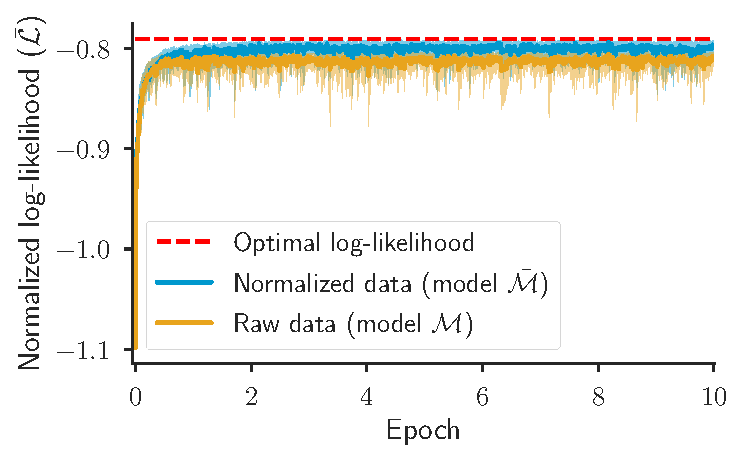
\includegraphics[width=0.3\textwidth]{../figures/SGD_norm_raw10.pdf}
        \label{fig:sgd_norm_unorm}
    }~
    \subfigure[Adagrad]{
        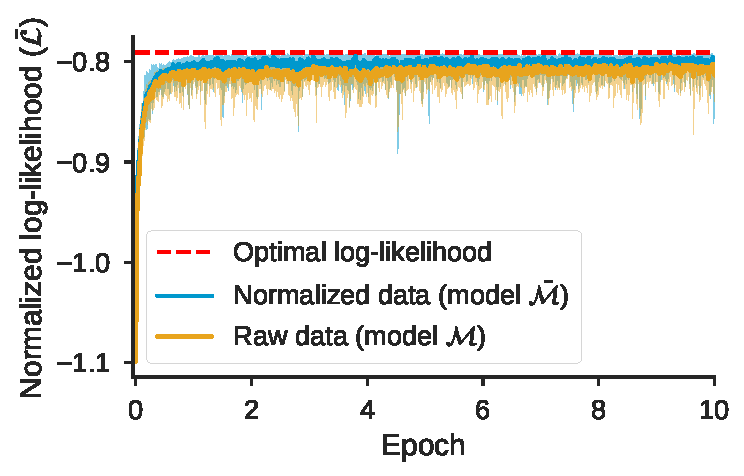
\includegraphics[width=0.3\textwidth]{../figures/adagrad_norm_raw10.pdf}
        \label{fig:adagrad_norm_unorm}
    }~
    \subfigure[SNM]{
        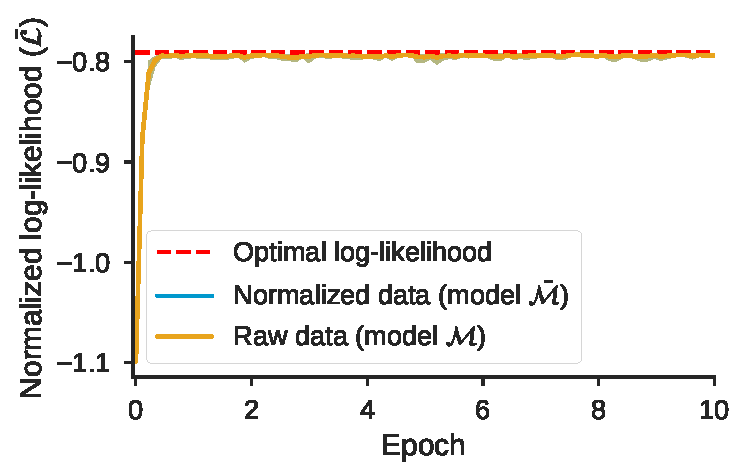
\includegraphics[width=0.3\textwidth]{../figures/SNM_norm_raw10.pdf}
        \label{fig:snm_norm_unorm}
    }
    \vspace{-0.2cm}
    \caption{Evaluation of the algorithms on raw data (model $\mathcal{M}$) and normalized data (model $\bar{\mathcal{M}}$). The vertical axis corresponds to the normalized log likelihood. Each time, ten runs have been executed. The lines correspond to the average value over all the runs, and the colored part corresponds to the 95\% confidence interval. SGD and Adagrad are run with a batch size of 100 observations, SNM is run with a batch size of 1,000 observations.}
    \label{fig:norm_unorm}
    \vspace{-0.5cm}
\end{figure*}

Figure \ref{fig:snm_norm_unorm} shows the results of the training on both models with SNM. We ran this algorithm with batches of 1,000 observations. Table \ref{tab:res_norm_unorm} shows the value of the normalized log-likelihood on the ill-conditioned model $\mathcal{M}$ and the normalized model $\bar{\mathcal{M}}$. Both the results from Figure \ref{fig:norm_unorm} and Table \ref{tab:res_norm_unorm} show that second-order methods have less problem with ill-conditioned optimization problem. Thus, it indicates that the information contained in the Hessian is important when the problem is ill-conditioned. Besides, we see that using a stochastic Hessian does not hurt the second-order methods when dealing with ill-conditioned problems.

\subsection{Comparison of the algorithms}
\label{sec:comp_algo}

At this point, we are interested in benchmarking the performance of SNM compared to other methods. The most used methods in the literature are the first-order methods and quasi-newton methods. Thus, comparing the optimization process of SNM against such methods can give us a good insight about the performance of our algorithm. Therefore, we first train SGD with different batch sizes, as well as gradient descent. The results are given in Figure \ref{fig:first_order}. We do the same for standard BFGS and RES-BFGS with batch sizes of 100 and 1,000. The results are given in Figure \ref{fig:quasi_newton}. Finally, we show the results for SNM. We trained it with two different batch sizes, 100 and 1,000, and we compare it against Newton method. The results are given in Figure \ref{fig:second_order}. For these three figures, we executed ten runs. Again, the lines give the average value for the normalized log likelihood, and the colored parts show the 95\% confidence interval.

\begin{table}[b]
\vspace{-0.5cm}
\centering
\renewcommand\arraystretch{1.2}
\begin{tabular}{l|ccc}
\multicolumn{1}{l}{} & {\bf SGD} & {\bf Adagrad} & {\bf SNM} \\ \cline{2-4}
on $\mathcal{M}$ & -0.808608 & -0.813525 & -0.793933 \\
on $\bar{\mathcal{M}}$ & -0.797970 & -0.801471
 & -0.793933 \\ \hline
rel. diff. & 1.33\% & 1.50\% & 0.00\%
\end{tabular}
\caption{\label{tab:res_norm_unorm} Average normalized log likelihood over a thousand runs at the tenth epoch for SGD, Adagrad, and SNM.}
\end{table}

\begin{figure*}[t]
\vspace{-1cm}
    \centering
    \subfigure[First-order methods]{
        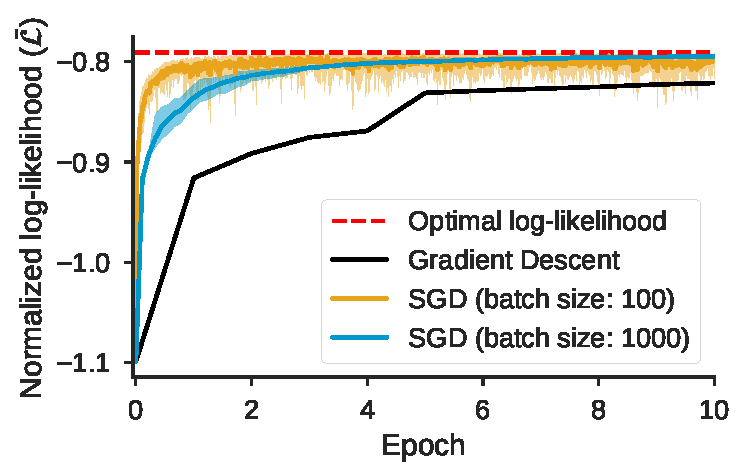
\includegraphics[width=0.3\textwidth]{../figures/SGD10.pdf}
        \label{fig:first_order}
    }~
    \subfigure[Quasi-Newton methods]{
        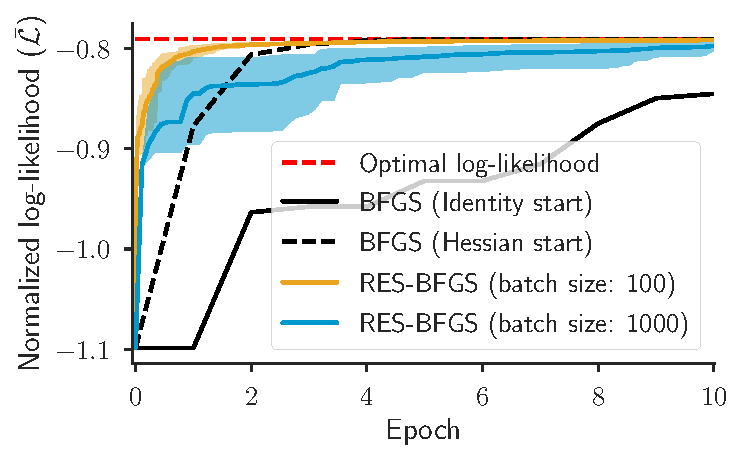
\includegraphics[width=0.3\textwidth]{../figures/SBFGS10.pdf}
        \label{fig:quasi_newton}
    }~
    \subfigure[Second-order methods]{
        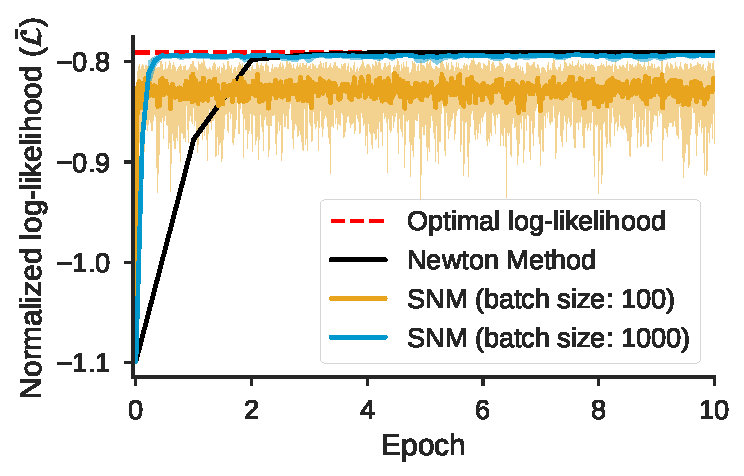
\includegraphics[width=0.3\textwidth]{../figures/SNM10.pdf}
        \label{fig:second_order}
    }
    \vspace{-0.2cm}
    \caption{Comparison of the different algorithms presented in Section \ref{sec:algorithms} and \ref{sec:snm}. The vertical axis corresponds to the normalized log likelihood. Each time, ten runs have been executed. The lines correspond to the average value over all the runs, and the colored part corresponds to the 95\% confidence interval.}
    \label{fig:comparison_algo}
    \vspace{-0.5cm}
\end{figure*}

\begin{table}
\centering
\renewcommand\arraystretch{1.2}
\begin{tabular}{lc|ccc}
&\multicolumn{1}{c}{batch} & {\bf first-order} & {\bf quasi-newton} & {\bf second-order} \\ \cline{3-5}
\multirow{ 2}{*}{\bf Stochastic} & 100 & -0.797970 & -0.791851 & -0.825096 \\
& 1000 & -0.794238 & -0.797552 & -0.793933 \\
\multicolumn{2}{l|}{\bf Full batch size}  & -0.821341 & -0.845372/-0.790806 & -0.790806
\end{tabular}
\caption{\label{tab:comparison_algo} Average normalized log likelihood over a thousand runs at the tenth epoch for first-order methods, quasi-newton methods, and second-order methods.}
\vspace{-1cm}
\end{table}

From Figure~\ref{fig:comparison_algo}, we see that first-order methods struggle the most in the early epochs. Then, we see that stochastic quasi-newton methods tend to struggle to reach the optimal value, especially with the first approximation of the Hessian being the identity matrix. Interestingly, we see that the RES-BFGS works better with smaller batch size while it tends to struggle and plateau with big batch size. Nevertheless, it can get closer to the optimal solution than SGD. However, SNM is the best algorithm out of the three regarding the log likelihood at the tenth epoch. Table \ref{tab:comparison_algo} gives the average value of the normalized log likelihood for the tenth epoch. In this table, we report two values for the quasi-newton method and the full batch size: the first value reported is with the first approximation of the Hessian being the identity matrix, the second value corresponds to the real Hessian. The numbers confirm that SNM is the best algorithm. However, it is interesting to note that contrary to the other two algorithms, SNM runs better with bigger batch size. In the next section, see Section~\ref{sec:effect_bs}, we study the possible reason behind such behavior.

\subsection{Effect of the batch size}
\label{sec:effect_bs}

As shown in Table~\ref{tab:comparison_algo}, for both SGD and SNM a more significant batch size works better than a smaller one. In this section, we are particularly interested about SNM, but the conclusion also holds for SGD. Firstly, we might think that it is because of constant switching between Newton step and gradient descent step. Indeed, the choice of the direction in the algorithm exploits the second-order information only if the batch hessian is positive (negative, if you maximize) definite. Thus, the larger the batch size, the higher the probability that it is the case. In Figure \ref{fig:perc_newton}, we show the percentage of Newton steps that the algorithm is performing as a function of the batch size. This percentage is computed on a thousand draws. \\

\begin{figure}[t]
\centering
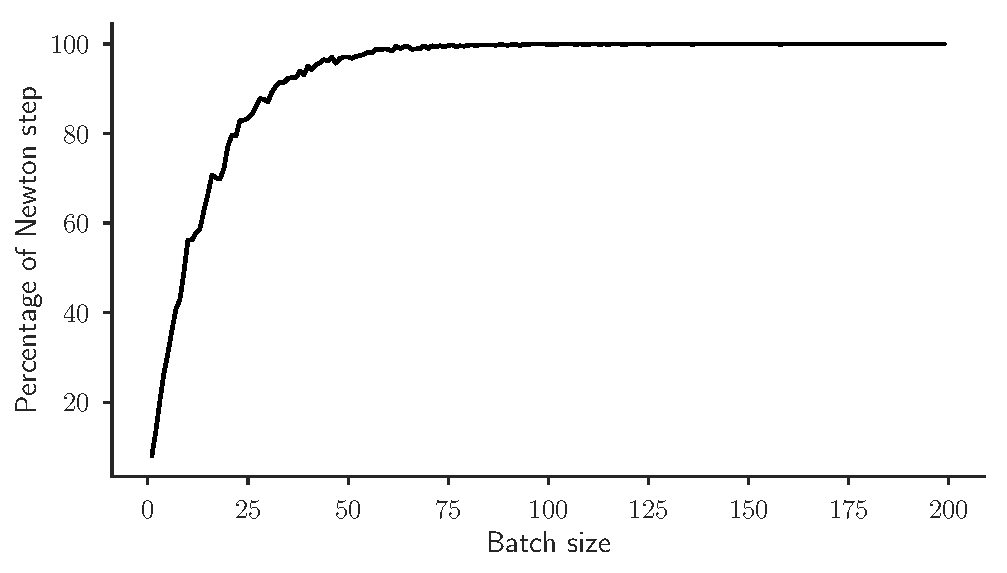
\includegraphics[width=0.37\textwidth]{../figures/perc_newton.pdf}
\vspace{-0.3cm}
\caption{Theoretical percentage of Newton step in function of the batch size for model $\bar{\mathcal{M}}$. The percentage was computed on a thousand draws.}
\label{fig:perc_newton}
\vspace{-0.3cm}
\end{figure}

As we can see, SNM tends to perform only Newton steps quickly. Indeed, with a batch of 100 observations, the algorithm performs a Newton step 99.86\% of the time. Therefore, the difference in the percentage of Newton steps between batches of 100 observations and batches of 1,000 observations is minimal. It leads to the conclusion that the issue aforementioned does not come from the switching between the two types of steps.

However, small batch sizes create other issues for all sorts of stochastic algorithms. Indeed, when computing the Hessian with small batch size, the only information we get is from a small subset of data. Therefore, for a given batch, the optimum can be different from the optimum on the whole dataset. Using the well optimized function \texttt{minimize} from the package \texttt{scipy.optimize}, we compute the optimum for different batch size. Then, we compare the euclidian distance between the optimum on the full dataset and the optimum from the different batches. Figure \ref{fig:batch_dist} shows the results of this experiment.

\begin{figure}[t]
\centering
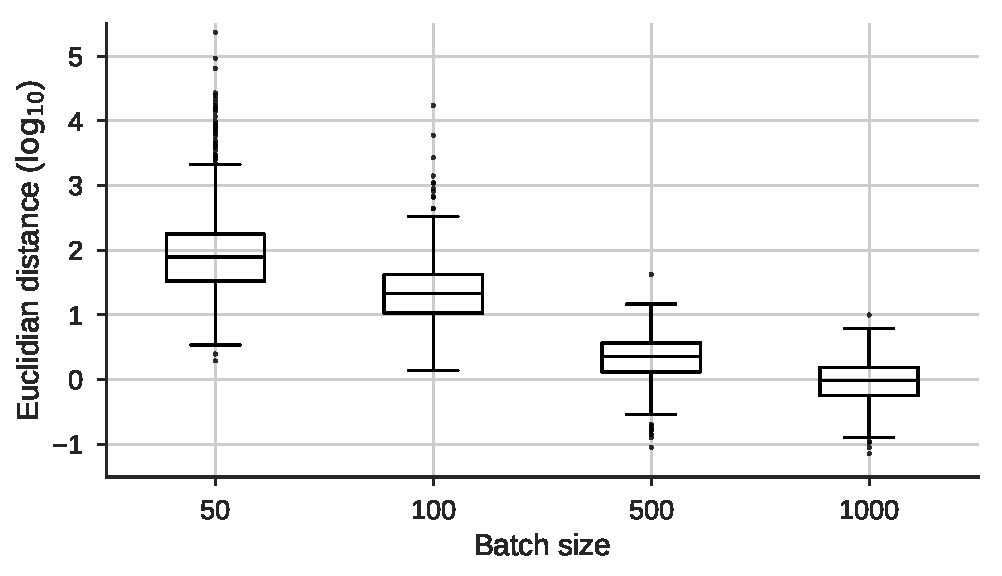
\includegraphics[width=0.37\textwidth]{../figures/dist.pdf}
\vspace{-0.3cm}
\caption{Euclidian distance between the optimal parameters obtained on the full dataset and optimal parameters found on batches of the data for different batch sizes. The line in the middle represents the median. A thousand draws were computed for each batch size.}
\label{fig:batch_dist}
\vspace{-0.5cm}
\end{figure}

In Figure~\ref{fig:batch_dist}, we see that when taking small batches, the optimal solution is pretty far from the optimal solution on all data points. Therefore, this creates a problem in the computation of the step for SNM. Indeed, since we do not take into account previous Hessian, as opposed to RES-BFGS, the algorithm will often change direction with small batches. Indeed, every time we change the batch, the algorithm is chasing a different optimum, making difficult for it to achieve the real optimum. 

Thus, one way to fix this kind of problem is to use variance-reduction techniques as done by the first-order method named SAG~\cite{schmidt_minimizing_2013}. Indeed, it would be interesting to accumulate second-order information from different batches in a pre-conditioning matrix. Such a matrix is more likely to be positive (negative for maximization) definite (we can enforce it if needed), and then used it to solve Newton's equations. 

\section{Conclusion}
\label{sec:conclusion}

In this paper, we have presented a second-order stochastic method called SNM.  Just as SGD methods, the central idea is to compute the Hessian on a batch of observations. While not possible for machine learning algorithms that are generally used for the estimation of models including millions of parameters,  we hypothesize that it is possible and desirable to include second-order information for estimating discrete choice models that generally contain no more than a dozen parameters. We showed that a second-order stochastic approach was legit thanks to the finite-sum shape of the log likelihood. We compared our algorithm with several first-order and quasi-newton benchmark algorithms using a simple discrete choice model. Preliminary results have revealed that (stochastic) first-order methods encounter issues in estimating the parameters of such models and that our algorithm was achieving better performances.  

Although preliminary results showed in this paper are encouraging, the current state of the algorithm only constitutes a first step toward our final goal that is the development of an optimization method specifically designed to estimate discrete choice model parameters on big data sets. The obvious next step is to use a more sophisticated way to calculate a pre-conditioning matrix using batch second order information. Also, the calculation of the step should be improved. Then, the theoretical properties of our approach need to be studied as the convergence rate of our algorithm is still unknown. Our algorithm will also have to be tested on more advanced discrete choice models (such as Nested Logit and Cross-Nested Logit models) and on much larger datasets. Regarding this latter, data sets including individuals' behavior over time have become increasingly available, and our approach seems to be particularly well suited for such data. Investigating the potential of our algorithm on panel data is therefore also an exciting avenue of future research. 

\section{Acknowledgements} 
\label{sec:acknowledgements}

We would like to thank Tim Hillel for his valuable insight on the development of this method as well as his comments that significantly improved this article.

\bibliography{PhD.bib}

\end{document}
